\documentclass[10pt]{SelfArx}
%\documentclass[10pt]{article}
\usepackage[T1]{fontenc}
\usepackage[utf8]{inputenc}

\usepackage{palatino}
\usepackage{upgreek}

%\PaperTitle{TITLE ON HEADER}
%  \PaperTitle{AI Instrumentation Institute (AI$^3$) for Discovery in Physics }
 
  \PaperTitle{ }

% Add packages and set options
\PassOptionsToPackage{usenames,dvipsnames}{xcolor}

%!TEX root = ./2017_NSF_proposal.tex
\AtBeginDocument{%
  \addtolength\abovedisplayskip{-0.5\baselineskip}%
  \addtolength\belowdisplayskip{-0.5\baselineskip}%
%  \addtolength\abovedisplayshortskip{-0.5\baselineskip}%
%  \addtolength\belowdisplayshortskip{-0.5\baselineskip}%
}



\usepackage{fec}
\usepackage[sort&compress]{natbib}
 \usepackage{comment}
\usepackage{graphicx}
\usepackage{multirow}
\usepackage{multicol}

% \RequirePackage{algorithmic,algorithm}




\newcommand{\tr}{\textrm{tr}}

\newcommand{\inTR}[1]{}
\newcommand{\setN}{N}

\usepackage{algorithm}
% \usepackage{algorithmic}
\usepackage{algpseudocode}

\usepackage[colorinlistoftodos,bordercolor=orange,backgroundcolor=orange!20,linecolor=orange,textsize=scriptsize]{todonotes}


%\usepackage[disable]{todonotes}



%\JournalInfo{\today} % Journal information
%\Archive{XXXX} % Additional notes (e.g. copyright, DOI, review/research article)


%\Authors{}
%\Keywords{} % Keywords - if you don't want any simply remove all the text between the curly brackets
\newcommand{\keywordname}{Keywords} % Defines the keywords heading name
%\Abstract{}


%\usepackage{subfigure}
%\usepackage{subfig}
\usepackage{enumitem}

\usepackage{epsfig}
\usepackage{color}
\usepackage{boxedminipage}
\usepackage{amsfonts}
\usepackage{amsmath}
\usepackage{url}

\usepackage{epstopdf}
\usepackage{enumitem}
\usepackage{natbib}
\usepackage{pdfpages}
\newcommand{\note}[1]{{\small \color{red} \it #1}}



\setlength{\bibsep}{0pt plus 0.3ex}
\setlength{\columnsep}{0.55cm} % Distance between the two columns of text
\setlength{\fboxrule}{0.75pt} % Width of the border around the abstract


%\usepackage{fontspec}
%\setmainfont{Arial}

 \newtheorem{theorem}{Theorem}
 \newtheorem{lemma}{Lemma}
% \newtheorem{propres}{Proposed Research}
%\newtheorem{propres}{Research Topic}
\newtheorem{propres}{Framework}

%---------------------------------------------------------------------------------------
%   COLORS
%----------------------------------------------------------------------------------------
\definecolor{color1}{HTML}{81071c} %   0,0,90  Color of the article title and sections
\definecolor{color2}{RGB}{0.972549,0.8352941, 0.5137255} % Color of the boxes behind the abstract and headings
\definecolor{light-gray}{gray}{0.1}
\color{light-gray}


%----------------------------------------------------------------------------------------
%   ABSTRACT
%----------------------------------------------------------------------------------------



\usepackage{epsfig}
\usepackage{epstopdf}

%----------------------------------------------------------------------------------------
%   HYPERLINKS
%----------------------------------------------------------------------------------------
% \usepackage{hyperref} % Required for hyperlinks

\newcommand\tagthis{\addtocounter{equation}{1}\tag{\theequation}}


\usepackage{amsmath}
\DeclareMathOperator{\Rand}{Rand}
\DeclareMathOperator{\support}{support}



% revision and comment
\usepackage[normalem]{ulem}
\usepackage[dvipsnames]{xcolor}
\newcommand{\del}[1]{{\ignorespaces \color{red} \sout{#1}}}
\newcommand{\add}[1]{{\color{blue} {#1}}}
\newcommand{\rewrite}[1]{{\color{SeaGreen} {#1}}}
\newcommand{\tored}[1]{{\color{red} {#1}}}



                       % such that
\newcommand{\ve}[2]{\left\langle #1 ,  #2 \right\rangle}    % inner product
\newcommand{\eqdef}{:=}
                    % set of real numbers
\newcommand{\Prob}{\mathbb{P}}                   % probability
                       % expectation

%\newcommand{\U}{U}
\newcommand{\argmin}{argmin}

\newcommand{\R}{ {\bf R}}
\newcommand{\Var}{\mathbf{Var}}
\newcommand{\hatZ}{\hat Z}
\newcommand{\hatS}{\hat S}
\newcommand{\calG}{G}
\newcommand{\calT}{\mathcal{T}}
\newcommand{\calF}{\mathcal{F}}
\newcommand{\Lip}{\mathcal{L}}
\newcommand{\calH}{\mathcal{H}_\beta}
\newcommand{\calHMINI}{\mathcal{C}}

\newcommand{\calS}{\mathcal{S}}
\newcommand{\calJ}{\mathcal{J}}
\newcommand{\x}{ {x}}
\newcommand{\y}{ {\bf y}}
\newcommand{\z}{ {\bf z}}
\newcommand{\vv}{ {\bf v}}
\newcommand{\wv}{ {\bf w}}
\newcommand{\av}{ {\bf \alpha}}
\newcommand{\bv}{ {\bf \alpha}}
\newcommand{\V}{ {\bf v}}
\newcommand{\T}{ {\bf T}}
\newcommand{\X}{ {\bf X}}

\newcommand{\0}{ {\bf 0}}
\newcommand{\alf}{ {\boldsymbol \alpha}}
\newcommand{\vchi}{ {\boldsymbol \chi}}

\newcommand{\vu}{{\bf u}}
\newcommand{\vdelta}{{\boldsymbol \delta} }
\newcommand{\w}{  {\bf w}}
\newcommand{\vt}{  {\bf t}}
\newcommand{\va}{  {\bf a}}

\newcommand{\f}{f}
\newcommand{\YY}{\varphi}
\newcommand{\K}{K}
\newcommand{\sK}{\mathcal{K}}
\newcommand{\J}{J}
\newcommand{\sJ}{\mathcal{J}}

\newcommand{\calO}{\mathcal{O}}
\newcommand{\vsubset}[2]{#1_{[#2]}}
\newcommand{\Srv}{\hat{S}}
\newcommand{\oo}{|J \cap \Srv_j|}

\newcommand{\vc}[2]{#1^{(#2)}}                   % coordinate of a vector
\newcommand{\cor}[2]{{{#1}_{#2}}}                   % coordinate of a vector
\newcommand{\corit}[3]{{#1}_{#2}^{(#3)}}                   % coordinate of a vector
\newcommand{\ncs}[2]{\|#1\|^2_{(#2)}}
\newcommand{\nbp}[2]{\|#1\|_{(#2)}}              % norm block primal
\newcommand{\nbd}[2]{\|#1\|_{(#2)}^*}            % norm block dual
\newcommand{\Rw}[2]{\mathcal R_{#1}(#2)}
\newcommand{\Rws}[2]{\mathcal R^2_{#1}(#2)}
        % Cardinality

\newcommand{\pnote}[1]{{  \color{red} [[ #1 -- Peter ]] }}
\newcommand{\natinote}[1]{{  \color{blue} [[ #1 -- Nati ]] }}
\newcommand{\takinote}[1]{{  \color{yellow} [[ #1 -- Martin ]] }}
\newcommand{\avnote}[1]{{  \color{green} [[ #1 -- Avleen ]] }}
\newcommand{\removed}[1]{}
\newcommand{\norm}[1]{\left\lVert{#1}\right\rVert}
\newcommand{\hingeloss}{\ell}
\newcommand{\hinge}[1]{\hingeloss ( #1 )}
\newcommand{\trans}{{\top}}
\newcommand{\calA}{\mathcal{A}}
\newcommand{\bP}{\mathcal{P}}
\newcommand{\bD}{\mathcal{D}}
\newcommand{\bH}{\mathcal{H}}
\newcommand{\sizeJ}{\omega}
\newcommand{\Gg}{\mathcal{G}^{\sigma'}}


\newcommand{\newstuff}[1]{{\color{red}#1}}
\newcommand{\cocoa}{\textsc{CoCoA}}
\newcommand{\cocoap}{\textsc{CoCoA$\!^{\bf \textbf{\footnotesize+}}$}}
\newcommand{\localalgname}{\textsc{LocalSolver}\xspace}
\newcommand{\localSDCA}{\textsc{LocalSDCA}\xspace}
\newcommand{\setn}{[n]}
\newcommand{\Exp}{\mathbb{E}}                      % expectation


\usepackage{caption}
\usepackage{subcaption}
%----------------------------------------------------------------------------------------
%   HYPERLINKS
%----------------------------------------------------------------------------------------
\usepackage{hyperref} % Required for hyperlinks
\hypersetup{colorlinks,breaklinks=true,urlcolor=color2,citecolor=color1,linkcolor=color1,bookmarksopen=false,pdftitle={Title},pdfauthor={Author}}

\graphicspath{{./}{./img/}}
\usepackage{ifthen}
\usepackage{calc}
\usepackage{pifont}
\usepackage{forloop}
\usepackage{wrapfig}
\usepackage{graphicx}
\usepackage[utf8]{inputenc}
%\usewrapackage{fontspec}
%\setmainfont{Arial}

%\usepackage{lineno}
%\linenumbers

\newcounter{starnumber}
\newcommand{\stars}[1]{
  \forloop{starnumber}{1}{\value{starnumber} < 4}{
    \ifthenelse{#1 < \value{starnumber}}{\ding{73}}{\ding{72}}%
  }
}
\usepackage[usenames,dvipsnames]{xcolor}
\usepackage{tcolorbox}
\usepackage{tabularx}
\usepackage{array}
\usepackage{colortbl}
\tcbuselibrary{skins}

\newcommand{\INPUT}{\textbf{Input}}
\newcommand{\FOR}{\textbf{For}~}
%\DeclareMathOperator*{\argmin}{argmin}

\newcolumntype{Y}{>{\raggedleft\arraybackslash}X}
 
%\tcbset{tab2/.style={enhanced,fonttitle=\bfseries,fontupper=\normalsize\sffamily,colback=yellow!10!white,colframe=red!50!black,colbacktitle=Salmon!40!white,coltitle=black,center title}}
\tcbset{tab2/.style={enhanced,fonttitle=\bfseries,fontupper=\normalsize\sffamily,colback=yellow!10!white,colframe=red!50!black,coltitle=black,center title}}

\usepackage{algorithm}
\usepackage{wrapfig}
\usepackage{hyperref}
% Seda did not want to have a blue links.... NSF also doesn't like it
%\hypersetup{colorlinks,urlcolor=blue}
 

\newcommand{\sups}[1]{{#1}}
\newcommand{\sss}[1]{{\scriptscriptstyle{#1}}}
 \usepackage[normalem]{ulem}

\newcommand{\hlt}[1]{{\color{red}\textbf{#1}}}
\newcommand{\hao}[1]{{\color{cyan}[Hao: \textbf{#1}]}}
\newcommand{\hlsfml}{{\tt hls4ml}}
\newcommand{\myparagraph}[1]{\noindent{\color{color1}\textbf{#1}}}

%**********
% Document
%**********

%\linespread{0.93}


\setlist[itemize]{leftmargin=5.5mm}


%\usepackage{lineno}
%\linenumbers



\begin{document}
\fontfamily{ppl}\selectfont





%Can be temporary, but useful for overall structure



%\tableofcontents
%\vspace{1cm}

%\begin{tabular}{c|c}
%Overview     & 1 \\
%Research 2.1     & 4.5 \\
%Research 2.2     & 4.5 \\
%Research 2.3     & 4.5 \\
%Intelec. Merit &  \\
%Broader impact &  \\ 
%Education     & 4 \\
%Broading     & 2.5 \\
%Knowledge Tr.     & 0.8 \\
%Management     & 1.5 \\
%Prior NSF     & 0.8 \\
%\hline 
%Total & 
%\end{tabular}




\clearpage


\begin{center}
{\bf \large 
Collaborative Research: CPS: Medium: Ultra Low Power Adaptive Inference for Autonomous Mobile Health 
}
\end{center}



\setcounter{page}{1}
\section{Overview}\label{sec.overview}
Unobtrusive monitoring of human activity within social and environmental context has far reaching applications across affective computing, mobile health, preventive medicine, and public health. 
Emerging CPS technologies offer platforms with rich multi modal sensing capabilities to support data-driven optimization and management of systems to help promote healthier lifestyles for individuals and larger populations, monitor distributions and spread of behaviors, person-to-person connectivity, infectious diseases, and even societal trends. 

A large number of these applications are driven by cyberphysical systems that require real-time responsiveness, ability to adapt and perform autonomous decision making, and perform reliable operation under stringent energy budgets. 
As we consider the closed loop of a cyberphysical system, these properties are necessary for all stages: (i) Sensors: As emerging CPS devices become increasingly powerful with growing modalities of sensing, the trade-offs between computation time and energy budgets is difficult to optimize. On one hand, there is a demand for omnipresent devices, yet, on the other hand, there is not enough energy and bandwidth to sustain them at large scale; 
(ii) Computation and Control of Physical Components: There are various reasons for increasing expectations of computational capabilities within CPS devices.
A prominent one concerns privacy. A device is generally considered more secure as it performs more of its analysis and decision making locally or closer to the source of the personal information. 
Another major reason is that, the responsiveness of the system would increase, if reasoning about the sensed environment/phenomenon is performed closer to the sensor and this would also allow for rapid adjustments to better focus on select aspects of the phenomenon in question. 
With these rising expectations energy budgets are easily being pushed beyond the currently available envelopes. 
Furthermore, off-the-shelf microprocessor-based platforms can neither match the required real-time latency nor the energy limits. 
To appropriate balance these trade-offs requires  co-development and optimization at the system, hardware, and algorithmic levels.

In this proposal, we aim to investigate co-design of machine learning hardware and algorithms for behavior monitoring applications and the integration of this AI/ML technology into cyberphysical systems to enable adaptive and intelligent capabilities constrained by the practical limitations of performance and energy efficiency. 
Our goal is to develop design methods and tools for enabling accurate inference capabilities to close the loop of the sensing and response cycles so that these CPS devices can process rich sensor data in real time for accurate inference, in resource constrained and dynamic environments. 
On one hand, it is desirable to perform majority of intelligent autonomous decisions and inference at the edge to alleviate privacy concerns as well as avoid excessive communication latencies that might render real-time closed loops infeasible. 
On the other hand, it is a challenge for ML-enhanced CPS devices to integrate sophisticated hardware for performing high speed inference within limited form factors and battery capacities. 
We will tackle this challenge by: 
(i) creating a co-design methodology that caters to the optimal design of specialized ML hardware for the needs of the CPS devices; 
(ii) embedding adaptive and reconfigurable features to the high performance ML hardware to create a solution that can be deployed at very large scale for low cost CPS devices; 
(iii) leveraging the adaptiveness of the underlying ML hardware so that it can accommodate a wide variety of sensors and facilitate nearly passive sensing behavior to achieve unprecedented energy efficiencies; 
and finally (iv) leverage transfer learning methods to adapt the same ML hardware to different sensing modes, behavior tracking contexts, and use cases.       




\section{Research Description}\label{sec.researchplan}

A Research Description that describes the technical rationale and technical approach of the CPS research, including the challenges that drive the research problem and how the research integrates cyber and physical components. This section must also describe how the research outcomes are translational to other application domains. Specifically, it must include:
A subsection titled "CPS Research Focus" which describes the cyber-physical system attributes of the challenge problem and clearly identifies the core CPS research areas addressed in which the novel and foundational research contributions are being made;

\subsection{CPS Research Focus}\label{sec:problems}
Basic application domain is daily life activity detection with social context, related to affective computing and mobile health. Basically outfit eyeglasses with multiple cameras (RGC and IR) that collect and understand what the wearer is doing and who they are meeting, and then sense biomarkers like blood pressure, electrodermal activity, head movement, eye movement, respiration rate, to map emotional state with interactions, which allows us to trigger interventions to help a patient (r.e. I detected your eating a bag of chips, you are on a diet, trigger intervention).

Glasses with hi-def raw images on them at 30FPS.
Thermal sensors
IMUs processing on multiple points across the eyeglasses.

Social sense and contact tracing? Facial recognition to count interactions? Privacy preserving on the device, capture behaviors.

Everything, including the obfuscation, and then the rough gesture recognition, and then the people interactions, on device.


\subsection{Application: Daily Life Activity and Interaction Detection}
Social interaction is a critical indicator for detecting certain mental health problems such as depression, PTSD, and anxiety. 
For clinicians and caregivers, understanding patient social interaction is critical for improving patient health outcomes and suggesting interventions and treatments. 
A convenient, accurate, usable, privacy respecting, and continuous solution for monitoring personal social interactions does not yet exist. MORE MOTIVATION FROM HEALTH. Insert STATS.

Social interaction is generally defined as the process that people act and react with others \cite{goffman1978presentation}. There have been several studies that show how social interaction impacts health markers, including stress \cite{ono2011relationship}, activity, and sleep quality. 
Increasing social interaction can positively impact a person, prevent certain mental health issues \cite{godart2000anxiety}, and can help reduce other health problems including stress, depression, and post-traumatic stress disorder \cite{vesnaver2011social}.

Current challenges include: (1) battery lifetime: we need weeks of lifetime while maintaining inference quality, (2) rich sensing and inference ability in real time, (3) lack of privacy for bystanders, which reduces wearer adherence and mental comfort.

We propose SocialCam, a low-power consumption wearable that continuously tracks the wearer's social interaction state. SocialCam integrates multiple forward facing RGB cameras into a pair of glasses as shown in \textit{Fig. \ref{glasses}}. Our device enables face detection and stereo vision based depth estimation. Additional sensors are used to sense and understand health biomarkers.  We propose a in-hardware inference pipeline that can continuously and automatically measure the wearer's social interaction state unobtrusively, conveniently, power-efficiently and without storing user's private data. 

\subsection{Essential Functions}
\begin{enumerate}
    \item Continuously capture personal bio-markers to understand personal health in the moment: including activity levels with IMUs, stress and anxiety via indirect methods including blood pressure via pulse transit time~\cite{}
    \item Capture faces / people in near field and far field using multiple imagers
    \item Understand attentiveness by observing the movement of the pupil
    \item Finally, obfuscate any collected images to preserve privacy of bystanders encountered by the wearer.
\end{enumerate}

\subsection{Device}
We propose a wearable eyeglass-style device that integrates two RGB cameras and a facial-recognition pipeline to detect the user's social interactions. No raw video data is ever retained, only records of the patient's social interactions. This enables a psychologist to monitor the user's social interactions through the data obtained by the device without compromising their privacy. 

Our system aims to collect meta-data about a user's socialization on a day-to-day basis for use in clinical settings; we are primarily interested in measuring how long users spend socializing in-person with others during the day. 
We assume that, for someone to be socializing with someone else in-person, social partners' faces must be in the user's line of sight. To directly measure faces in the user's line of sight, our wearable system consists of an eyeglass frame outfitted with two low-power, forward facing RGB cameras. 
To enable stereo vision based depth estimation, the cameras will be spaced 100 - 140mm apart near the uppers corners of the eyeglass frame. Unlike monocular chest-mounted systems, our system implicitly follows the user's line of sight, is capable of incorporating stereo-vision depth information into analyses, and is more discrete because it fits naturally into normal eyewear.


Outfitting users always-on stereo cameras presents serious privacy and data storage challenges; the vast majority of recorded data will be irrelevant, taking up storage space and - more importantly - compromise user privacy and make users feel uncomfortable \cite{alharbi2018can}. To overcome all of these issues, almost all data processing occurs on-system. As soon as images are captured, facial recognition is performed and relevant metadata is collected. No sensitive user images are ever stored or transmitted. The only data that ever leaves the platform is anonymized social interaction statistics.

Face detection will be carried out by a machine learning pipeline implemented on Lattice iCE40 FPGAs, and resulting statistics will be stored in on-board FRAM. We arbitrarily choose the left camera to be used for facial recognition. When faces are recognized in the image stream from the left camera, a stereo-vision depth estimation algorithm is run on the ROIs where faces were detected in the left image stream. The system will be powered by a 3.7V LiPo battery. Our system does not need to operate at a high frame rate, so we only process images at 0.2 - 0.5Hz to save power.

The primary challenge in designing this system is limiting power consumption. The hardware composition and energy consumption of each part in SocialCam is shown in \textit{Fig. \ref{hardware}}. The glasses need to be worn for 16 - 24 hour periods to be clinically useful, but battery capacity is limited by user comfort. Commercial eyewear systems like the Google Glass have a reported battery capacity of about 2,000 mAh \cite{muensterer2014google}. If we limit ourselves to half of that battery capacity and target a system runtime of 20 hours, our power draw is limited to 185mW. Data-sheets and white-papers from manufacturers suggest that this power envelope is achievable. We plan to use HiMax HM01B0 image sensors, which only require 2mW to operate at 30FPS and 320x240 resolution \cite{hm01b0}. Estimating power consumption for FPGAs is difficult because their power consumption is heavily design-dependent, however Lattice claims that human face detection is possible using less than 1mW \cite{latticeAI}, and recent work claims power consumption of about 5mW when evaluating their very small, 2-layer, 16-neuron, deep neural net about 1.1 million times per second \cite{roukhami2019very}. With these figures, our proposed system with two HM01B0 cameras, one FPGA for monocular face detection on the left camera and a second for stereo depth perception would consume less than 15mW, nearly an order of magnitude less than our target power consumption.


\subsection{ML Methods}\label{sec:ML}



\subsection{Hardware Co-Design}\label{sec:hardware}
Powerful AI instrumentation relies on {\bf co-design} -- the idea that system constraints, algorithm development, and hardware implementation inform and guide each other in complementary ways. 
%Development of physics experiments are typically driven by this principle which starts from the physics requirements and drills down to the technical specifications of the apparatus. 
AI\textsuperscript{3}'s co-design ecosystem is illustrated in Fig.~\ref{fig:codesign}. In addition to hard real-time latency constraints, other experimental challenges provide further constraints.  For example, sensors in harsh and complex environments may have strict power limits or need to operate in high radiation or cyrogenic environments.  Therefore, we will explore hardware co-design for various technologies from FPGAs to custom integrated circuits like ASICs and neuromorphic chips to ultra-low power photonics and opto-electronic devices to exotic memristive and organic-electronic hybrids. 


\subsubsection{Algorithm-Architecture Co-Design} \label{sec:HwAlgo}

\begin{wrapfigure}{r}{0.5\textwidth}
\centering
\vskip-40pt
  {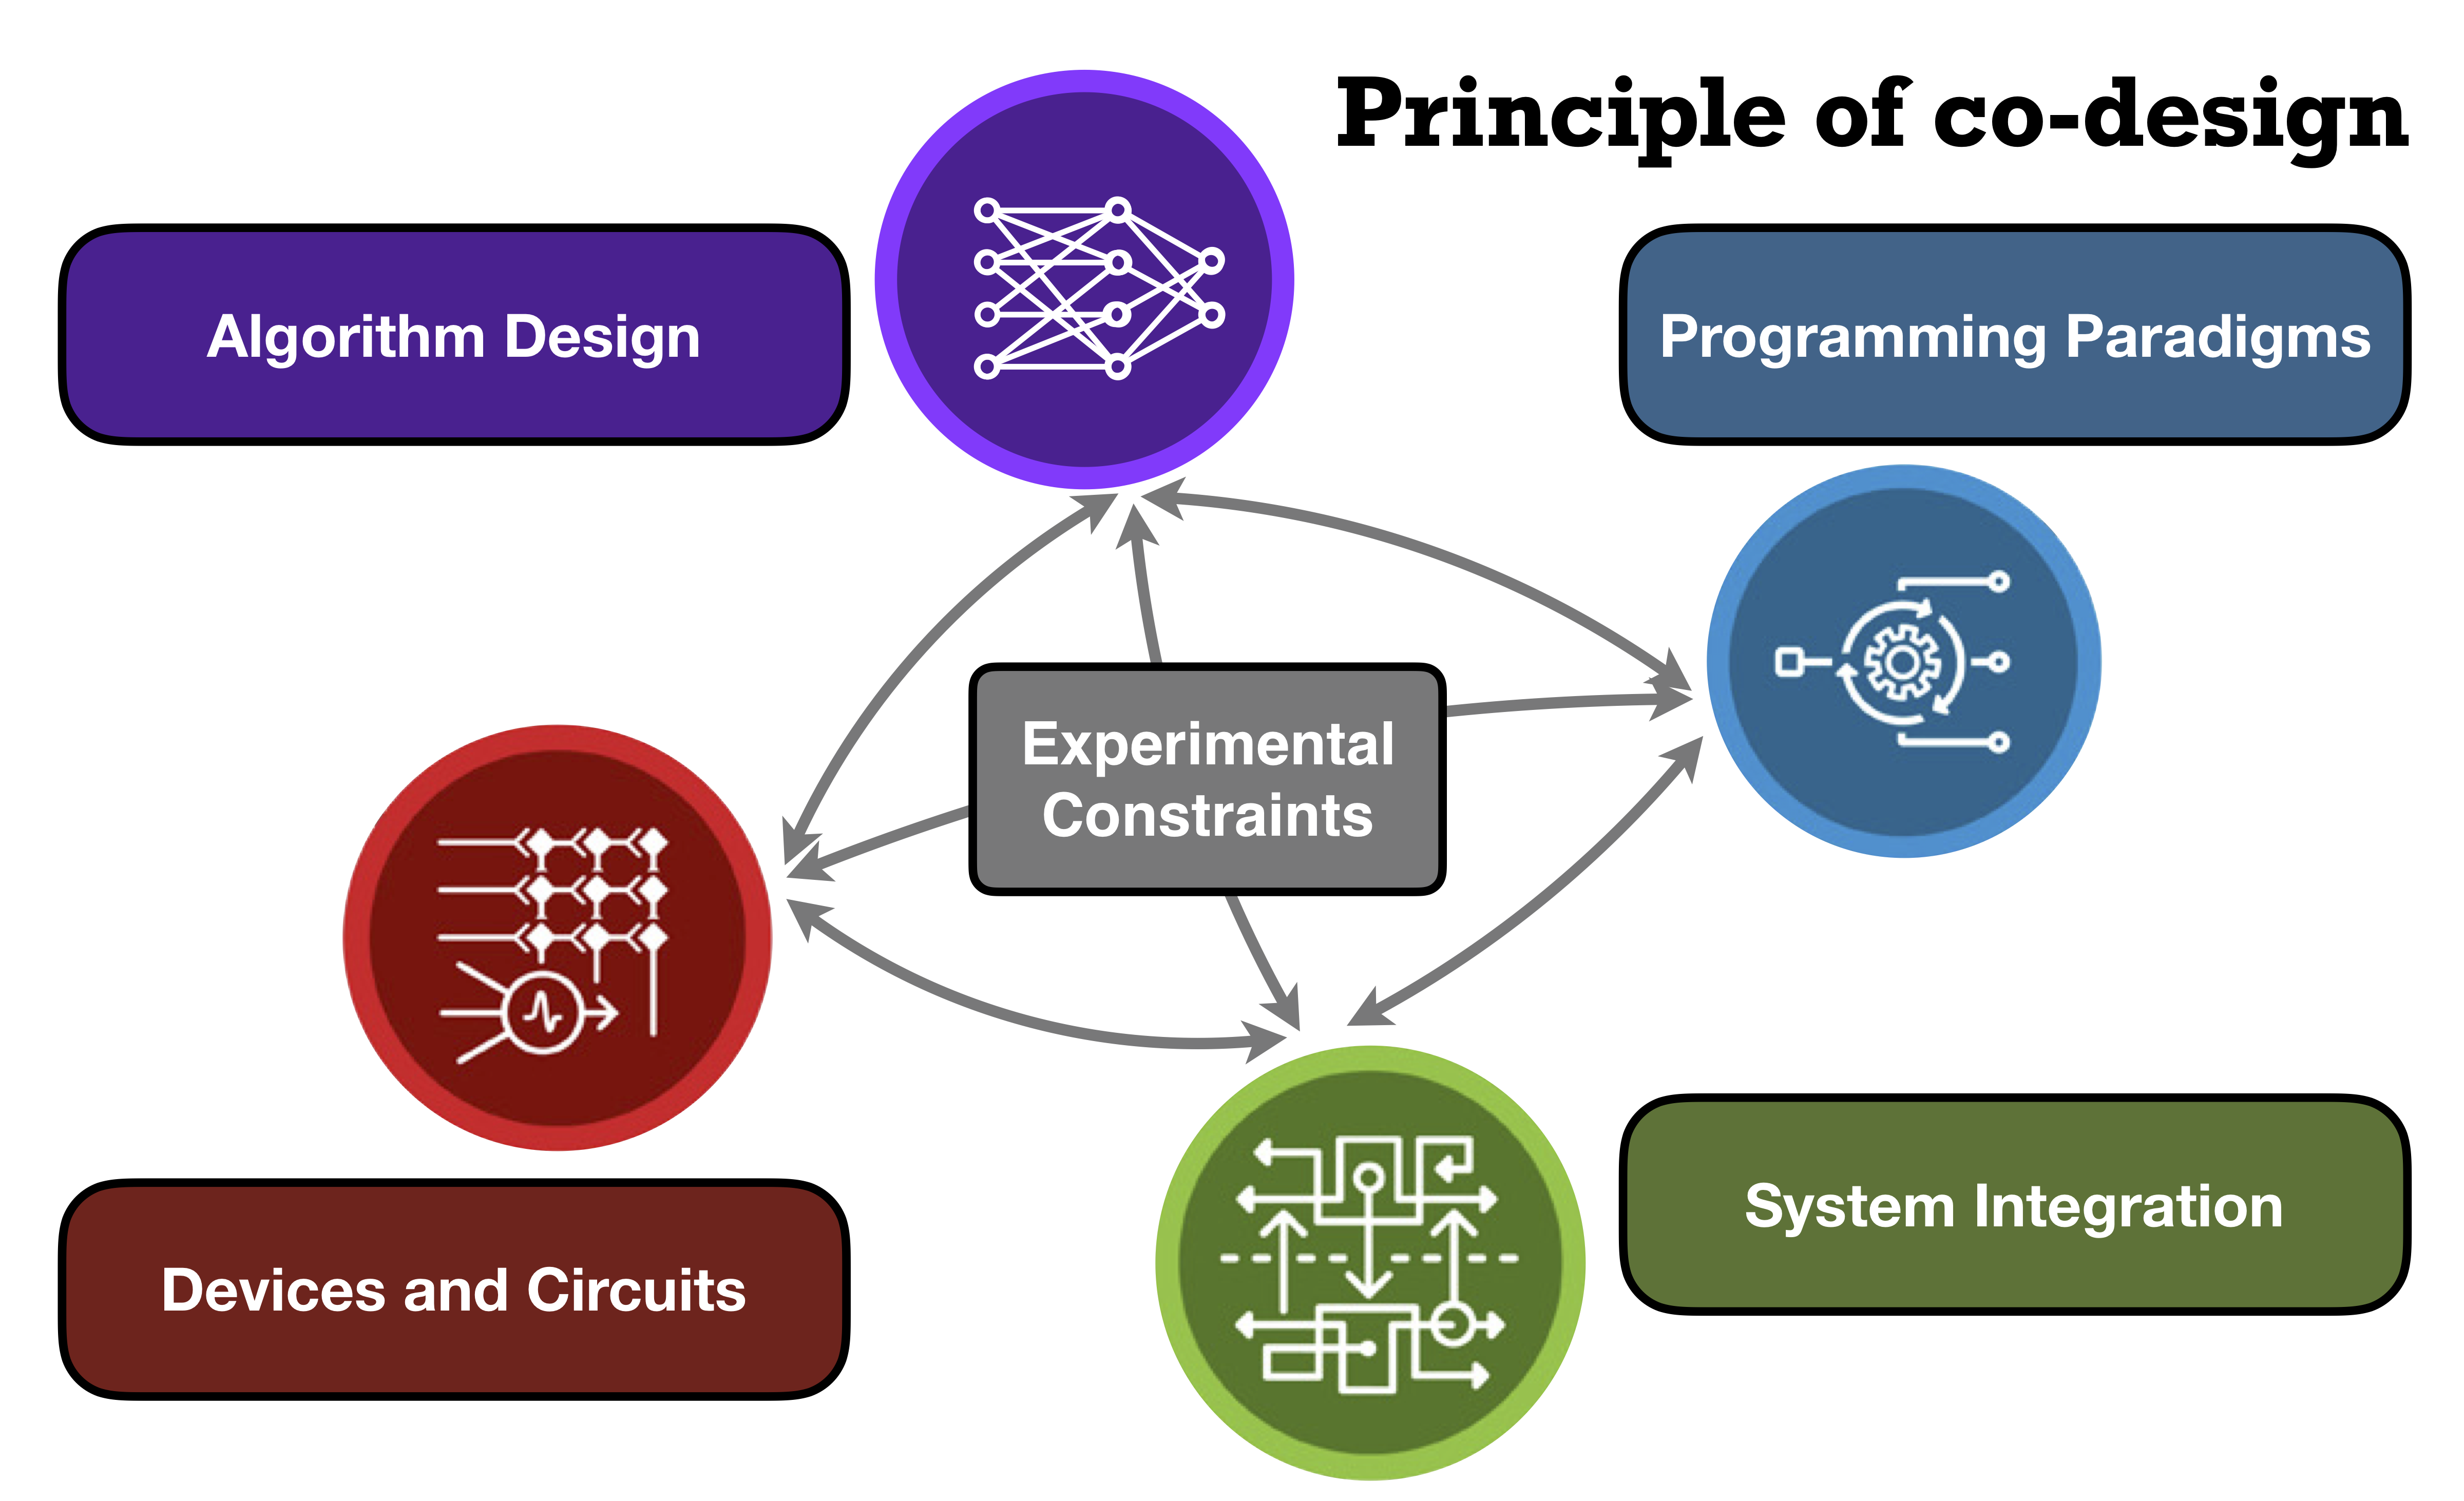
\includegraphics[keepaspectratio, width=0.5\textwidth]{proposal/img/codesign.png}}
  \caption{Hardware co-design principle which coherently integrates all levels of experimental design.}
  \label{fig:codesign}
  \vskip-15pt
\end{wrapfigure}
The development of efficient AI implementations in hardware begins with algorithm performance and design.
%Section~\ref{sec:AI} details the many AI methods that are required to attain our significant physics goals.  
As we consider how to implement the AI hardware in high-rate and resource-constrained environments, there are important considerations in building the most efficient systems. We must consider the size and structure of the AI computation. Neural networks are generally characterized through a number of multiplication and addition operations using fitted parameters (weights) determined during the training procedure. By reducing both the number of mathematical operations and how often the weights need to be accessed, the algorithm can be made more efficient.  Further, the precision at which the calculations are performed is also important.
%The optimization of the number of operations and their precision and the number of parameters can greatly reduce the resources required to perform a given AI computation.  
{\bf SP Duarte} and collaborators~\cite{Duarte:2018ite} explored the design space of AI algorithm performance while reducing the calculation precision and removing unimportant calculations (pruning/compression).  However, as neural network architectures become more complex and varied, this optimization must be understood in greater detail. New techniques, such as energy-aware pruning, can be used to improve the energy consumption directly~\cite{DBLP:journals/corr/YangCS16a}.

Just as important is the conception of the AI architecture. AI algorithms are over-parameterized universal function approximators. Directly connected to our research of physics-inspired learning (see Section~\ref{sec:AI}),  embedding our own physics knowledge into the neural network design can drastically reduce the number of parameters in a given neural network algorithm.  For example, exploiting physical symmetries in neural networks has been shown to reduce the computational complexity, e.g., tensor field networks that incorporate rotation- and translation-equivariance for 3D point cloud data~\cite{thomas2018tensor}. {\bf SP Su's} work has also demonstrated that learning a spectral convolutional neural network may achieve isometric invariance of geometric data. 

In order to create optimal AI hardware implementations, both of the above techniques are required.  First, we can reduce the computational complexity of the AI algorithm by embedding our physics knowledge into the network design. Then, we can further optimize the efficiency by adapting the algorithm for custom hardware while minimizing the energy footprint of calculation and maintaining performance. A central aspect of AI\textsuperscript{3}'s research program is to understand the strengths and limitations of different AI algorithms and techniques (from physics-inspired networks to transfer learning, compression, and autoencoders), including their ultimate performance, computational complexity, and applicability in hardware. {\bf SP Duarte} will lead this project in collaboration with {\bf SP Su}.

%%%%%%%%%%%%%%%%%%%%%%%%%%%%%%%%%%%%%%%%%%%%%%%%%%%%%%%%%%%%%%%%%%%%%%%%%%%%%%%%%%%%%%%%%%%%%%%
%%%%%%%%%%%%%%%%%%%%%%%%%%%%%%%%%%%%%%%%%%%%%%%%%%%%%%%%%%%%%%%%%%%%%%%%%%%%%%%%%%%%%%%%%%%%%%%

%\newpage 
\subsubsection{Programming Paradigms and Tools} \label{sec:Programming}


\begin{wrapfigure}{r}{0.6\textwidth}
\centering
\vskip-15pt 
  %\fbox
  {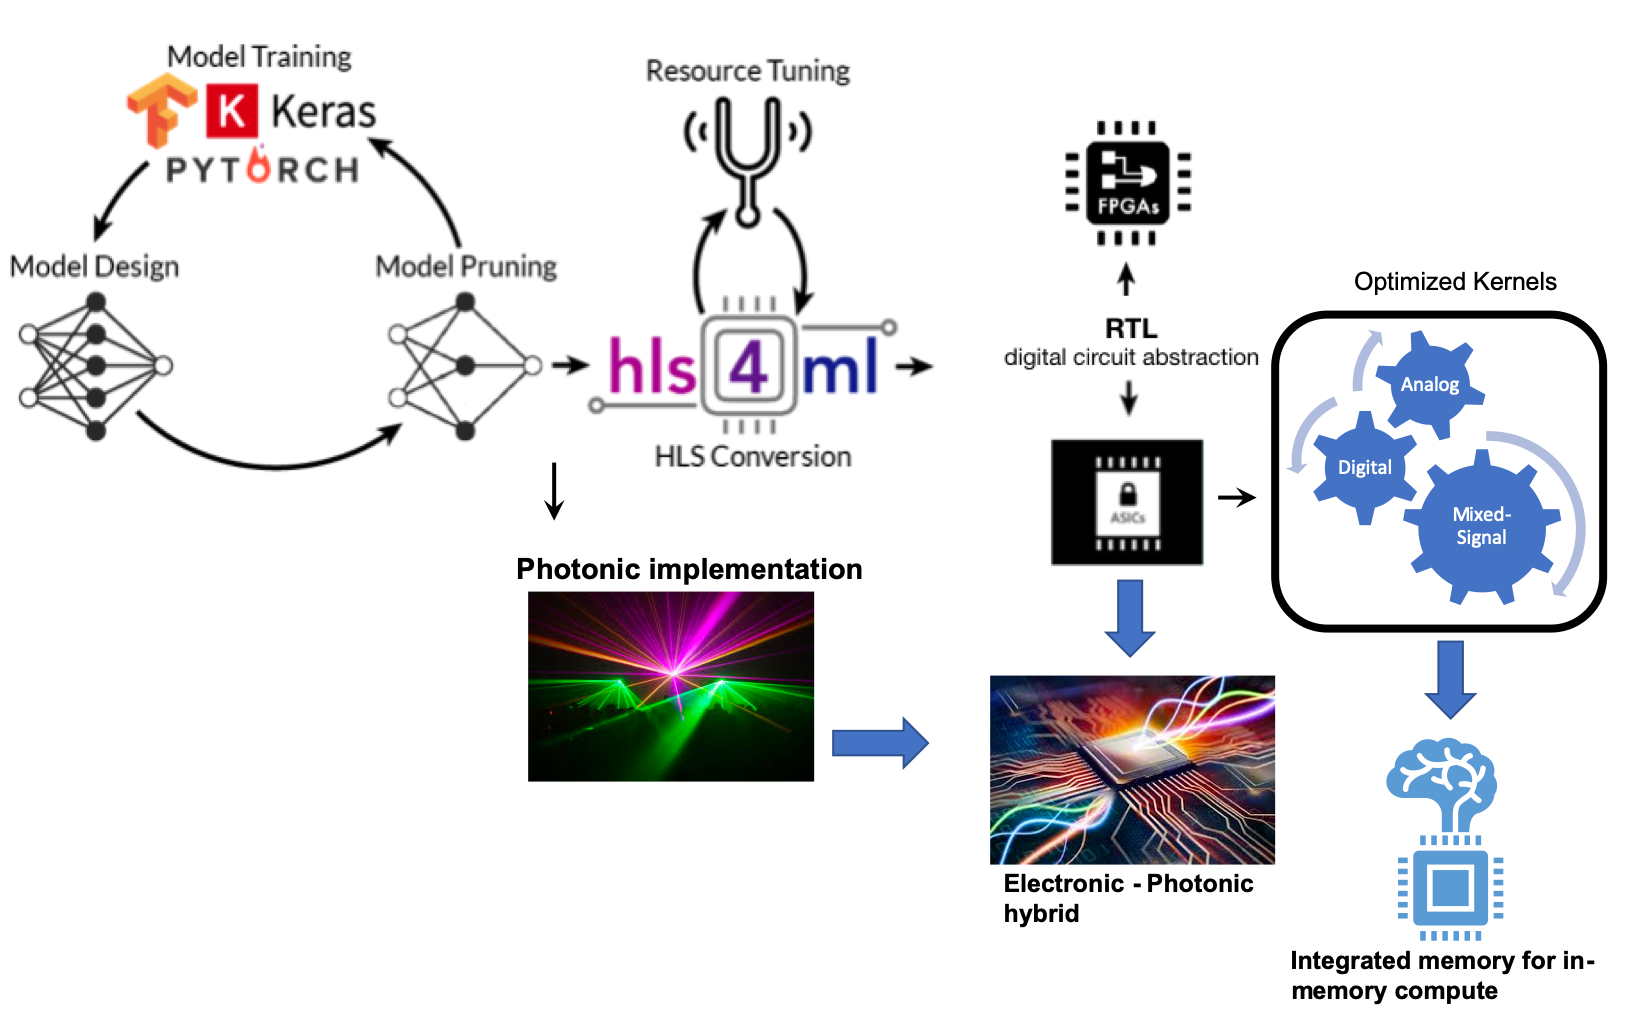
\includegraphics[keepaspectratio, width=0.6\textwidth]{proposal/img/ProgrammingFlow.png}}
  \caption{Full example workflow from HLS programming paradigms to hybrid solutions.}
  \label{fig:programming}
  \vskip-10pt 
\end{wrapfigure}
AI\textsuperscript{3}'s main goal in developing programming paradigms and tools will be to increase accessibility of hardware implementations of  algorithms in order to accelerate the development cycles for AI instrumentation. Mature programming tools are absolutely vital to wider deployment and adoption which will in turn improve the overall physics design process. Furthermore, widely accessible programming paradigms will be instrumental for easy and quick adoption by a large community of learners that can be trained for the future workforce in AI instrumentation for physics. %AI\textsuperscript{3} is targeted towards experimental physics constraints, but the tools will be available to the entire design automation community and for developing solutions in other domains. In that regard, 
AI\textsuperscript{3} will also be responsible for communicating, supporting, and educating developers and users. 
%Our plans on translating AI\textsuperscript{3}'s innovations on tool building and methodologies to the broader community will be further discussed in Section~\ref{sec.collab}.   


We will align our tool development strategies with the unique aspects of AI computation. One of the key features of neural networks are their modularity. This allows us to develop programming paradigms that enable the developer to separate and recombine these specific modular units to build larger neural network architectures. The basic description of the AI circuit implementation, for example, can be in a register-transfer language (RTL), but each kernel would be configurable based on resource, latency, and bandwidth constraints.   
%The integration of the kernels into a cohesive system is the subject of the next section on system design and integration, Section~\ref{sec:Integration}. 
One important aspect to AI\textsuperscript{3}'s research program is the use of higher-level programming paradigms based on low-level hardware representations.  
%Programming languages such as High Level Synthesis (HLS) and OpenCL are {\tt C}-based languages which are used to convert code into Register Transfer Level (RTL) Hardware Description Language (HDL). 
\textbf{SP Duarte} is one of the leading developers of a tool called \hlsfml~\cite{Duarte:2018ite} which takes popular open-source machine learning software frameworks such as {\tt TensorFlow}, {\tt Keras}, and {\tt PyTorch} and converts their model descriptions into high-level synthesis (HLS) code. The HLS code has parameters which tune the performance of the underlying hardware description to customize it for different system constraints.  The \hlsfml~tool then uses HLS tools to create an RTL-HDL description of a given AI algorithm for a specific type of hardware.  Despite being a new software package, this tool has seen widespread adoption in the HEP community and has been successfully used for fully-connected neural networks in LHC trigger applications on FPGAs.  The full workflow of \hlsfml~is depicted in Fig.~\ref{fig:codesign}. \textbf{SPs Hahn and Memik} have also been collaborating in developing HLS-based design methodologies for mapping the TrackletEngine algorithm used as part of Level-1 trigger track finding for CMS at the HL-LHC. 
  %This collaboration led to a better understanding of performance bottlenecks when using a commercial FPGA HLS tool flow and the co-PIs will be transferring their experience on existing HLS flows targeting HEP applications to \textbf{co-PI Duarte's} lab as they explore new programming paradigms suited for this domain collectively.  
While developing HLS tools for AI computation in hardware is an important research goal, HLS is not the only solution for AI algorithm implementation.  
%We will explore the limitations of this approach and develop alternatives, as well as compare them to other published software tools, such as Nengo which is described below. 
We plan to extend the workflow in Fig.~\ref{fig:programming} to allow for different types of AI algorithm kernels, domains, and hardware. As an example, EM applications require recurrent neural network structures to optimally interpret their time-ordered data; and \hlsfml~does not yet support those types of recurrent structures.  Further, to support the entire community, it is necessary to support other hardware types.  This includes other custom designs, i.e., Photonic Integrated Circuits (ICs), Digital and  Mixed Mode ASICs. ASICs are particularly important across physics because often experimental instrumentation must operate in extreme and harsh environments, such as high radiation and cryogenics, and off-the-shelf FPGAs are not feasible.  In the case of ASICs, specifically, there is no existing mature tool openly available for physics. This workflow can be further extended to less mature but potentially paradigm shifting technologies (see Section~\ref{sec:circuits}).  As such technologies become more mature, making them available to the developer is important for their deployment. {\bf Memik and Tran} will co-lead the development of AI-hardware tool flows.


%%%%%%%%%%%%%%%%%%%%%%%%%%%%%%%%%%%%%%%%%%%%%%%%%%%%%%%%%%%%%%%%%%%%%%%%%%%%%%%%%%%%%%%%%%%%%%%
%%%%%%%%%%%%%%%%%%%%%%%%%%%%%%%%%%%%%%%%%%%%%%%%%%%%%%%%%%%%%%%%%%%%%%%%%%%%%%%%%%%%%%%%%%%%%%%

\subsubsection{System Design and Integration} \label{sec:Integration}
%This aspect of co-design cycle is dedicated to 
Solutions will be needed for integration of the AI implementations into a coherent experimental system, including: {\bf interfacing} AI kernels to components such as power and memory management, device infrastructure and controls, and networking protocols; {\bf communication} with other devices in both a homogeneous and heterogeneous hardware stack; {\bf software interfaces} with the operators and users for features such as neural network weight programmability and neural network training and feedback loops.
%\begin{itemize}
%[noitemsep,topsep=0pt]
%    \item AI kernels to components such as power and memory management, device infrastructure and controls, and networking protocols
%\end{itemize}    

%\begin{itemize}[noitemsep,topsep=0pt]
%    \item Communication with other devices in both a homogeneous and heterogeneous hardware stack
 %   \item Software interfaces with the operators and users for features such as neural network weight programmability and neural network training and feedback loops
%\end{itemize}

An example of a conceptual system which requires all three aspects listed above is shown in Fig.~\ref{fig:reinforce}.
Here, a dynamical reinforcement learning system is depicted for a generic system which controls an experimental apparatus. It could be a realistic representation for particle physics, photon synchrotrons, and scanning EM.
In this system, a system-on-chip device which contains both an FPGA and a ARM-based CPU is deployed.  This system is communicating with a high-speed data acquisition system, which is aggregating the data in large offline storage to develop a complex surrogate model.  The target model for controlling the experiment is shown in the red box labeled "Target Model".  Batches of data are recorded and used to continue training the model based on the desired reward.  The system then requires both an interface for the ARM core with the external developer and a way for the ARM system which is training the model to update the weights in the target model.  This all requires the Target Model kernel to be interfaced with the rest of the FPGA firmware infrastructure. While this is a simplified example, it illustrates multiple system interfaces.


%%%%%%%%%%%%%%%%%%%%%%%%%%%%%%%%%%%%%%%%%%%%%%%%%%%%%%%%%%%%%%%%%%%%%%%%%%%%%%%%%%%%%%%%%%%%%%%
\subsubsection{Devices and Circuits} \label{sec:circuits}
\begin{wrapfigure}{r}{0.6\textwidth}
\centering
\vskip-20pt
  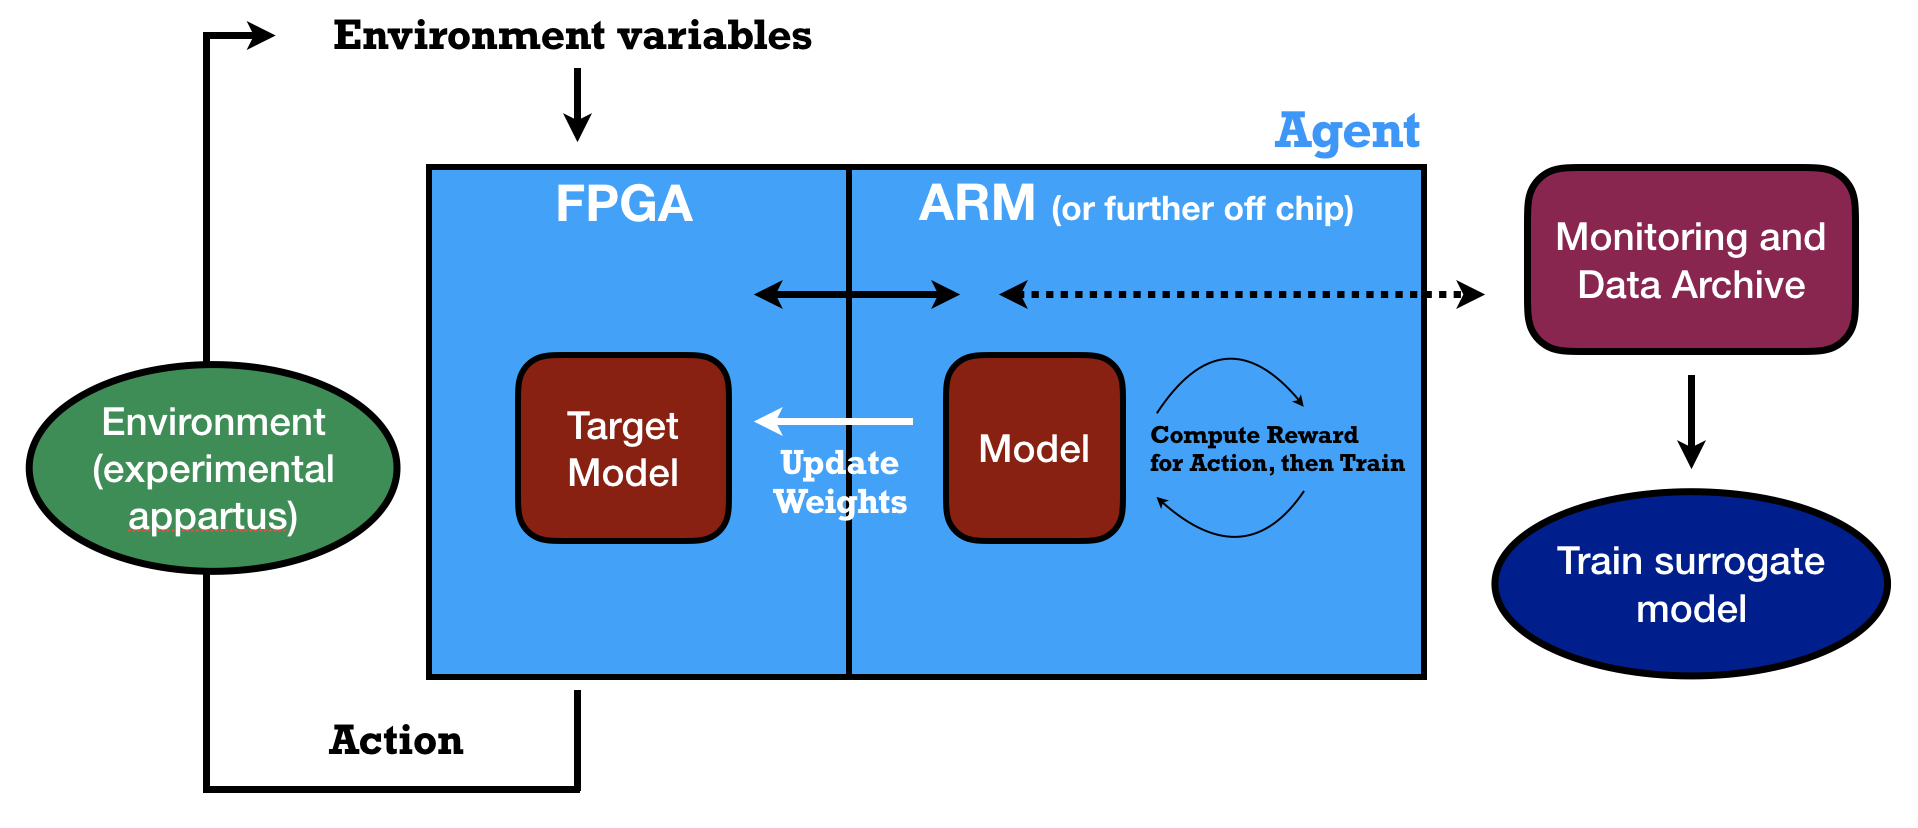
\includegraphics[keepaspectratio, width=0.6\textwidth]{proposal/img/reconfigurableArch.png}
  \caption{An example of a dynamically reconfigurable system}
  \label{fig:reinforce}
\vskip-10pt
\end{wrapfigure}
ML algorithms have been quite successfully implemented with digital hardware, so we do not plan to compete with the traditional, heavily resourced digital design companies, such as Intel and IBM, in developing AI and neuromorphic hardware. Nonetheless, commercial digital systems will have significant roles to play in AI\textsuperscript{3} research: in the short-, and mid-range goals, we plan to rely on digital platforms, such as FPGAs and digital ASICs, to realize the novel AI systems in this proposal. 

These systems will be co-designed with the algorithm developers and physics experimentalists in order to optimize their efficiency for the planned AI\textsuperscript{3} problems. As a result, AI\textsuperscript{3} will produce a stack of technologies for immediate, intermediate, and long-term solutions and workforce training. Our ability to span this stack of options will reduce the risks associated with each of these technologies when used alone. We plan to develop digital AI hardware that will be co-designed with the experiments to optimize the throughput and decision making in real-time.  To design the relevant AI algorithms that can be executed on our hardware, we plan to use and extend tools resulting from our research program, such as extensions to hlsfml~\cite{Duarte:2018ite} (see Section~\ref{sec:Programming}), for fast prototyping of algorithms. 
% add citations for Stewart, 2009; Bekolay, 2014; Lin, 2018]
%add citations to (Eliasmith, 2003, 2005)



\myparagraph{FPGA-based fast prototyping.} 


\myparagraph{Digital ASICs.}
ASICs are ideal for implementing integrated  on-detector low power and low latency edge computation. Power consumption due to data transfer from pixel to the chip periphery
%and subsequently off-chip 
dominates the total power consumed by ROICs. Hence locally analyzing data and extracting features not only efficiently utilizes data bandwidth, but also creates a smart detector.  There exist ASICs with highly parallel, modular sub-structures such as Google TPUs. However, co-design with the physics algorithms allows an extremely efficient, integrated, individually optimized kernel based approach for synthesizing complex interconnections. These interconnections allow extensive inter-regional (group of sensing elements) communication such that data analysis has a global view instead of just highly parallel local self-contained approach. 



\textbf{SP Memik} will lead the effort on implementing a holistic biologically-inspired retinomorphic approach where various individually optimized modules could be co-designed based on the AI algorithms. Designs will be fabricated in a fully depleted silicon-on-insulator (SOI) process (e.g. 22 FDX) for low power, high speed performance due to its lower parasitic capacitance. To achieve the ultimate power efficiency the digital circuits will be designed to operate in deep sub threshold regions with supply voltages of 200~mV or lower. Tool flows developed in Sec.~\ref{sec:Programming} will be utilized to convert AI algorithms to synthesizable Verilog for implementation. Standard CAD tools from vendors such as Cadence, Synopsys, Mentor Graphics etc. will be used to design, verify and create GDS II files for manufacture.  ASICs will be fabricated using dedicated multi-project wafer runs offered by several design aggregation service providers such as Globalshuttle, MOSIS, MUSE etc.








 
\section{Evaluation/Experimentation Plan}\label{sec.evalplan}



%\section{Intellectual Merit}\label{sec.intellectual}

\section{Broader Impacts}\label{sec.broaderimpact}


%\section{Education and Workforce Development}\label{sec.education}

%\section{Broadening Participation Plans}\label{sec.broadpar}
AI\textsuperscript{3}'s efforts will be organized in multiple avenues as follows:



\myparagraph{Broadening Participation for Undergraduate Students.} As program-level leaders and members of the admissions committees (\textbf{SP Memik is the Director of the Computer Engineering Program at NU} in various graduate programs, and diversity committees at all partner institutions, we have contributed to increasing the number and percentage of women and minority substantially. 
%Under \textbf{Etienne-Cummings' leadership} at JHU, students have access to the Education, Outreach and Diversity Committee (composed of faculty, students and staff) to influence local decisions, organize events and resolve conflicts. We believe that our past success in recruiting and retaining women and under-represented minorities is due to providing an intellectually challenging but supporting environment. 

\textbf{SP Agar} will partner with a minority serving institution, Morgan State University, to teach his interdisciplinary course on Data Analysis and ML there remotely. 

%We will also organize a day-long tour of the Fermi National Laboratories for local undergraduate student members of The Society of Women Engineers, The National Society of Black Engineers, and the Society of Hispanic Professional Engineers. By experiencing the nation's leading particle physics and accelerator laboratory in person, the students will develop an interest in the needs of the physics discoveries that drive AI\textsuperscript{3}.

\myparagraph{Broadening Participation for Graduate Students.}
SPs will implement recruitment and retention initiatives through all graduate programs relevant to AI\textsuperscript{3} research. At NU, \textbf{Memik} is also a faculty leader of the Graduate Women in Computing Group and a founding member of Diversity Committees in both the ECE and CS Departments. 

In order to connect the graduate programs of the AI\textsuperscript{3} partners with URM+W students, the institute will maintain a strong presence at conferences with diversity focus. \textbf{Memik} has been organizing a booth for NU-CS and CE programs at the Grace Hopper Celebration for Women in Technology for the past three years. Following that model, booths will be staffed exclusively by the PIs representing their programs at the URM-W focused conferences such as the SACNAS National Diversity in STEM Conference, ACM Richard Tapia Celebration of Diversity of Computing, Grace
Hopper Celebration of Women in Computing, and the National Society of Black Engineers Convention. Expo participants at these events are provided access to the resume databases of the attendees. We will leverage this access to network with students to advertise our outreach events and recruit into our research programs. 

%\textbf{SPs Takac and Agar} will be actively seeking funding to develop a larger exhibit at a large museum (e.g. in NYC) to bring the excitement of this cross-disciplinary work to as broad an audience as possible.

\myparagraph{Other Public Outreach.} We will leverage venues such as the Science Cafes to interact with the general public. 

\myparagraph{Measuring Progress.} 
%\section{Project Management and Collaboration Plan}\label{sec.collab}


\section{Project Management and Collaboration Plan}\label{sec.mangtplan}
Our team is comprised of 
{\bf Seda Memik} is an expert on power and thermal-aware circuit and system design, and design automation. \textbf{Memik} has strong ties with the physics instrumentation in HEP. She contributed to the first prototype chip for the Endcap Timing Readout Chip developed for the CMS Endcap at HL-LHC~\cite{Liu:2019twepp}. She was involved in the late stage power and thermal modeling for the VIPRAM2D ASIC as part of a CMS L1 Tracking Trigger demonstration~\cite{Deptuch:2289503}. She has taken critical leadership roles, managing teams of faculty and collaborating with School-, and University-level administration. 
She was the Director of Graduate Studies for the former EECS Department (overseeing six graduate programs, MS and PhD in CS, CE, EE). 
She is currently the Director of the Computer Engineering Division under the ECE Department. 
She served on the University-wide Limited Submissions Committee between 2016-2019, overseeing NU-wide competition for limited submission to the most prestigious research awards of the nation. 
%She is also an elected member of the School of Engineering Promotion and Tenure Committee for the next two years and also a member of the Faculty Board for the NU Keyman Modern Turkish Studies.     


\textbf{Joshua Agar}
is an expert in the development of multichannel spectroscopy techniques in quantum materials.\cite{Pandya2019-ma,Ievlev2018-sw,Saremi2018-py,Agar2018-ew,Ievlev2018-uq, Ievlev2018-us,Damodaran2017-mv,Damodaran2017-ve,Agar2016-fx,Pandya2016-hy,Damodaran2016-dk,Agar2016-ys,Zhang2015-oz,Agar2015-sv,Agar2014-ds,Mangalam2013-ne,Mangalam2013-tw,Karthik2013-zm,Karthik2012-ad}
Agar has been leading a new wave of interdisciplinary researchers who deploy ML in science. 
%This work includes creating a custom featurization protocol for the detection of enhanced nanoscale electromechanical energy conversion in $PbZr_{0.2}Ti_{0.8}O_{3}$,\cite{Agar2018-ew,Agar2019-eq} and deploying deep neural networks (DNNs) to understand ferroelectric switching, conductive domain wall behavior, and electron energy loss spectroscopies (EELS).\cite{Agar_undated-wi,noauthor_undated-ib,Agar_undated-wi}
%Agar has ongoing efforts to deploy novel DNN architectures to extract information from experimental data and to accelerate the search for new functional materials.\cite{Agar_undated-yi,Agar2018-zu} 
Agar is actively involved in promoting open reproducible science. He is a contributor to open-source Python libraries for the storing and analysis of multidimensional scientific data (pycroscopy\cite{Somnath2018-yp} and pyUSID\cite{Somnath2018-yp}. Agar has set a new precedent for publication by including with manuscripts the data, analysis codes, and executable Jupyter notebooks papers that allow for text, code, and descriptions to be evaluated, understood and repurposed. 
As a Cross-Cutting Lead he will be responsible for coordinating the efforts in physics and fundamental AI. 




\section{Results from Prior NSF Support}

\myparagraph{Seda Memik:} CCF-1422489:HF:Small:Thermal Monitoring in 3D Integrated Circuits, \$450,000, 7/15/2014-6/30/2018; 
{\bf Intellectual Merit:} A thin film bimetallic thermocouple technology for temperature sensing, including fabrication methods and chip integration is developed. {\bf Broader Impact:} Detailed real-time thermal mapping will allow significant improvements in dynamic monitoring for energy-efficient computers with greater computational power. This will benefit the sustainability of future computing systems. This project has resulted in a Ph.D. thesis~\cite{daweiThesis}, a book~\cite{Memik2016HeatMI}, and publications~\cite{LiTVLSI,LiDAC2017,LiISCAS}.




\newpage

%\bibliographystyle{plain}
\bibliographystyle{unsrt}

% JD: inserted this bib format as it's common in HEP, but I'm not sure what the best format is for NSF proposals, so feel free to change it back.
%\bibliographystyle{lucas_unsrt}

% PLEASE DO NOT CHANGE CITATION STYLES!!!!!! NSF has a strict rules....!!! :))))

% THANKS

\bibliography{literature,prior_takac,prior_choudhary_agrawal}


\end{document}